\documentclass[11pt]{article}
\usepackage[fontset=none]{ctex}
\usepackage{tcolorbox}
\usepackage{framed}
\usepackage{multirow}
\usepackage{setspace}
\usepackage{tikz}
\usetikzlibrary{shapes,decorations}
\usepackage{ulem} % 下划线
\usepackage{float} % 借助float包的H选项使tbox内可以插入表格
\usepackage{geometry}
\geometry{b4paper,landscape,left=0.2cm,right=1.1cm,top=1.5cm,bottom=2cm}
\usepackage{fancyhdr} %设置页码
\usepackage{lastpage} %获取总页数
\pagestyle{fancy} %fancyhdr宏包新增的页面风格
\renewcommand\headrulewidth{0pt} %取消页眉中的装饰分割线
\fancyhf{}
\cfoot{\footnotesize \qquad 第 \thepage\ 页 \quad 共 \pageref{LastPage}页}% 第X页 共Y页

\setmainfont{Times New Roman}
\setCJKmainfont{SimSun}[BoldFont=FandolSong-Bold, ItalicFont=STXingkai] % 中文字体

\newcommand{\s}{\uline{\qquad \qquad \qquad \qquad} \quad} % 短横线
\newcommand{\m}{\uline{\qquad \qquad \qquad \qquad \qquad \qquad \qquad \qquad \quad \ } \quad} % 中横线
\renewcommand{\u}{\uline{\hfill}} % 长横线

\linespread{1.8}


\begin{document}

    \begin{minipage}{0.477\linewidth}
        \begin{tcolorbox}[left=0.5mm,right=0.5mm,height=21.5cm,colback=white,boxrule=0.5pt]
        \begin{center}
            {\large \bfseries 志成中学 2022-2023 学年九年级第一次模拟考试}

            % {\large \bfseries 语文答题卡}
            \smallskip

            考号：\underline{ \qquad \qquad} \quad 姓名：\underline{ \qquad \qquad} \quad 考场：\underline{ \qquad \qquad} \quad 座号：\underline{ \qquad \qquad}
        \end{center}
    \vspace{-10pt}

\begin{spacing}{1.5}
    \begin{table}[H]
        \begin{tabular}{|l|c|}
        \hline
        \multicolumn{1}{|c|}{注意事项}                                                                                                                                                                      & \multirow{3}{*}{} \\ \cline{1-1}
        \begin{tabular}[c]{@{}l@{}}{\scriptsize 1.   答题前请将姓名、班级、考场、座号和准考证填写清楚。}\\      {\scriptsize 2. 客观题答题，必须使用2B铅笔填涂，修改时用橡皮擦干净。}\\      {\scriptsize 3. 主观题必须用黑色签字笔书写。}\\      {\scriptsize 4. 必须在题号对应的答题区域内作答，超出答题区域书写无效。\qquad \qquad \qquad \qquad \qquad }\\      {\scriptsize 5. 保持答卷清洁完整。}\end{tabular} & \qquad  \quad ~~贴条形码区  \qquad \quad  \qquad \\ \cline{1-1}
        正确填涂 \qquad  
        \fcolorbox{black}{black}{\parbox[c][0.05cm]{0.4cm}{~}}  \qquad    缺考标记   \qquad  \fcolorbox{black}{white}{\parbox[c][0.05cm]{0.4cm}{~}}   &        \\ \hline
        \end{tabular}
        \end{table}
\end{spacing}

    \vspace{-10pt}
    {\bfseries 第一部分(47分)}
    \vspace{-10pt}
    \begin{framed}

    1. (每空1分) (1) \s (2) \s (3) \s 

    \quad (4) \s (5) \s \s

    2. (每空1分) (1) \s \s 
    
    \quad (2) \s \s

    3. (3分) \s
    
    4. (3分) \s
    
    5. (1) (2分) \u

    \u

    \quad (2) (2分) \u
    
    \u

    \quad (3) (3分) \u
    
    \u

    \u
\end{framed}


\end{tcolorbox}
\end{minipage}\hfill
\begin{minipage}{0.477\linewidth}
    \begin{tcolorbox}[left=0.5mm,right=0.5mm,height=21.5cm,colback=white,boxrule=0.5pt]
        
    {\bfseries 第二部分(47分)}
    \vspace{-10pt}
    \begin{framed}
        6. (2分) \s
        
        7. (2分) \u

        \u

        \u

        8. (2分) \u

        \u

        \u

        9. (每空1分) (1) \s (2) \s 

        \quad (3) \s (4) \s

        10. (3分) 逆\ 旅\ 人\ 有\ 妾\ 二\ 人\ 其\ 一\ 人\ 美\ 其\ 一\ 人\ 恶\ 恶\ 者\ 贵\ 而\ 美\ 者\ 贱。

        11. (2分) \s

        12. (1) (2分) \u

        \u

        \quad (2) (2分) \u
        
        \u

        13. (2分) \u

        \u    
        
        \u

        14. (3分) \u

        \u    
        
        \u

        15. (3分) \u

        \u

    \end{framed}

    \end{tcolorbox}
\end{minipage}

\begin{minipage}{0.477\linewidth}
    \begin{tcolorbox}[left=0.5mm,right=0.5mm,height=21.5cm,colback=white,boxrule=0.5pt]
        \begin{framed}
            16. (3分) \u

            \u    
            
            \u

            \u

            17. (3分) \u

            \u    
            
            \u

            \u

            18. (2分) \u

            \u    
            
            \u

            \u
            
            19. (2分) \u

            \u    
            
            \u

            \u
            
            20. (3分) \u

            \u    
            
            \u

            \u
            
            21.  (1) (1分) \u

            \u
    
            \quad (2) (1分) \u
            
            \u

    
        \end{framed}
    
        \end{tcolorbox}
\end{minipage}\hfill
\begin{minipage}{0.477\linewidth}
    \begin{tcolorbox}[left=0.5mm,right=0.5mm,height=21.5cm,colback=white,boxrule=0.5pt]
        \begin{framed}
            

            21.  (1) (1分) \u

            \u
    
            \quad (2) (1分) \u
            
            \u

            22. (3分) \u

            \u    
            
            \u

            \u

            23. (2分) \u

            \u    
            
            \u
    
            \u

        \end{framed}
    
        \end{tcolorbox}
\end{minipage}


\begin{minipage}{0.477\linewidth}
    \begin{tcolorbox}[left=0.5mm,right=0.5mm,height=21.5cm,colback=white,boxrule=0.5pt]
    {\bfseries 第三部分(50分)}
\vspace{4pt}

\begin{center}
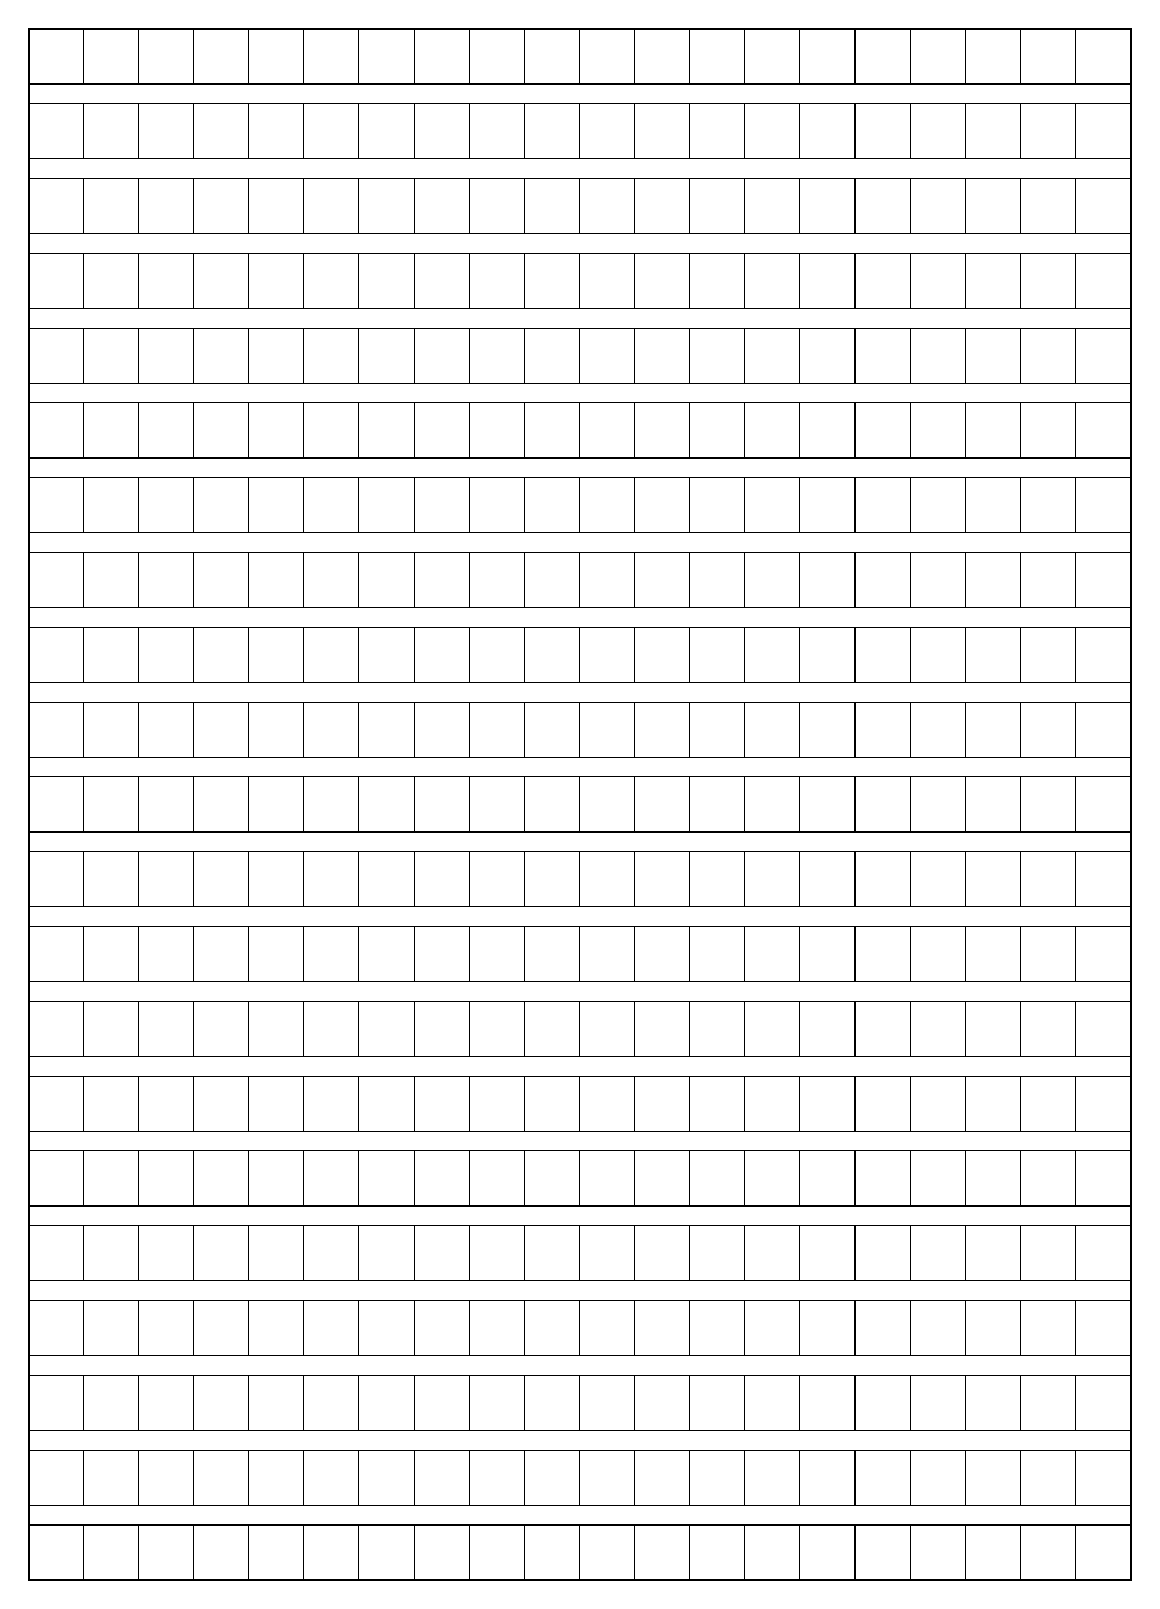
\begin{tikzpicture}[scale=1,x=0.7cm,y=0.95cm]
    \foreach \x [count=\xi] in {1,2,...,20}
    \foreach \y [count=\yi] in {1,2,...,21}
    \node[anchor=east,draw,minimum size=0.7cm]at(\x,\y){};%$\y$
    \draw[thick](0,0.63)rectangle(20,21.37);
    \end{tikzpicture}
\end{center}
    \end{tcolorbox}
    \end{minipage}\hfill
    \begin{minipage}{0.477\linewidth}
    \begin{tcolorbox}[left=0.5mm,right=0.5mm,height=21.5cm,colback=white,boxrule=0.5pt]
        \begin{center}
            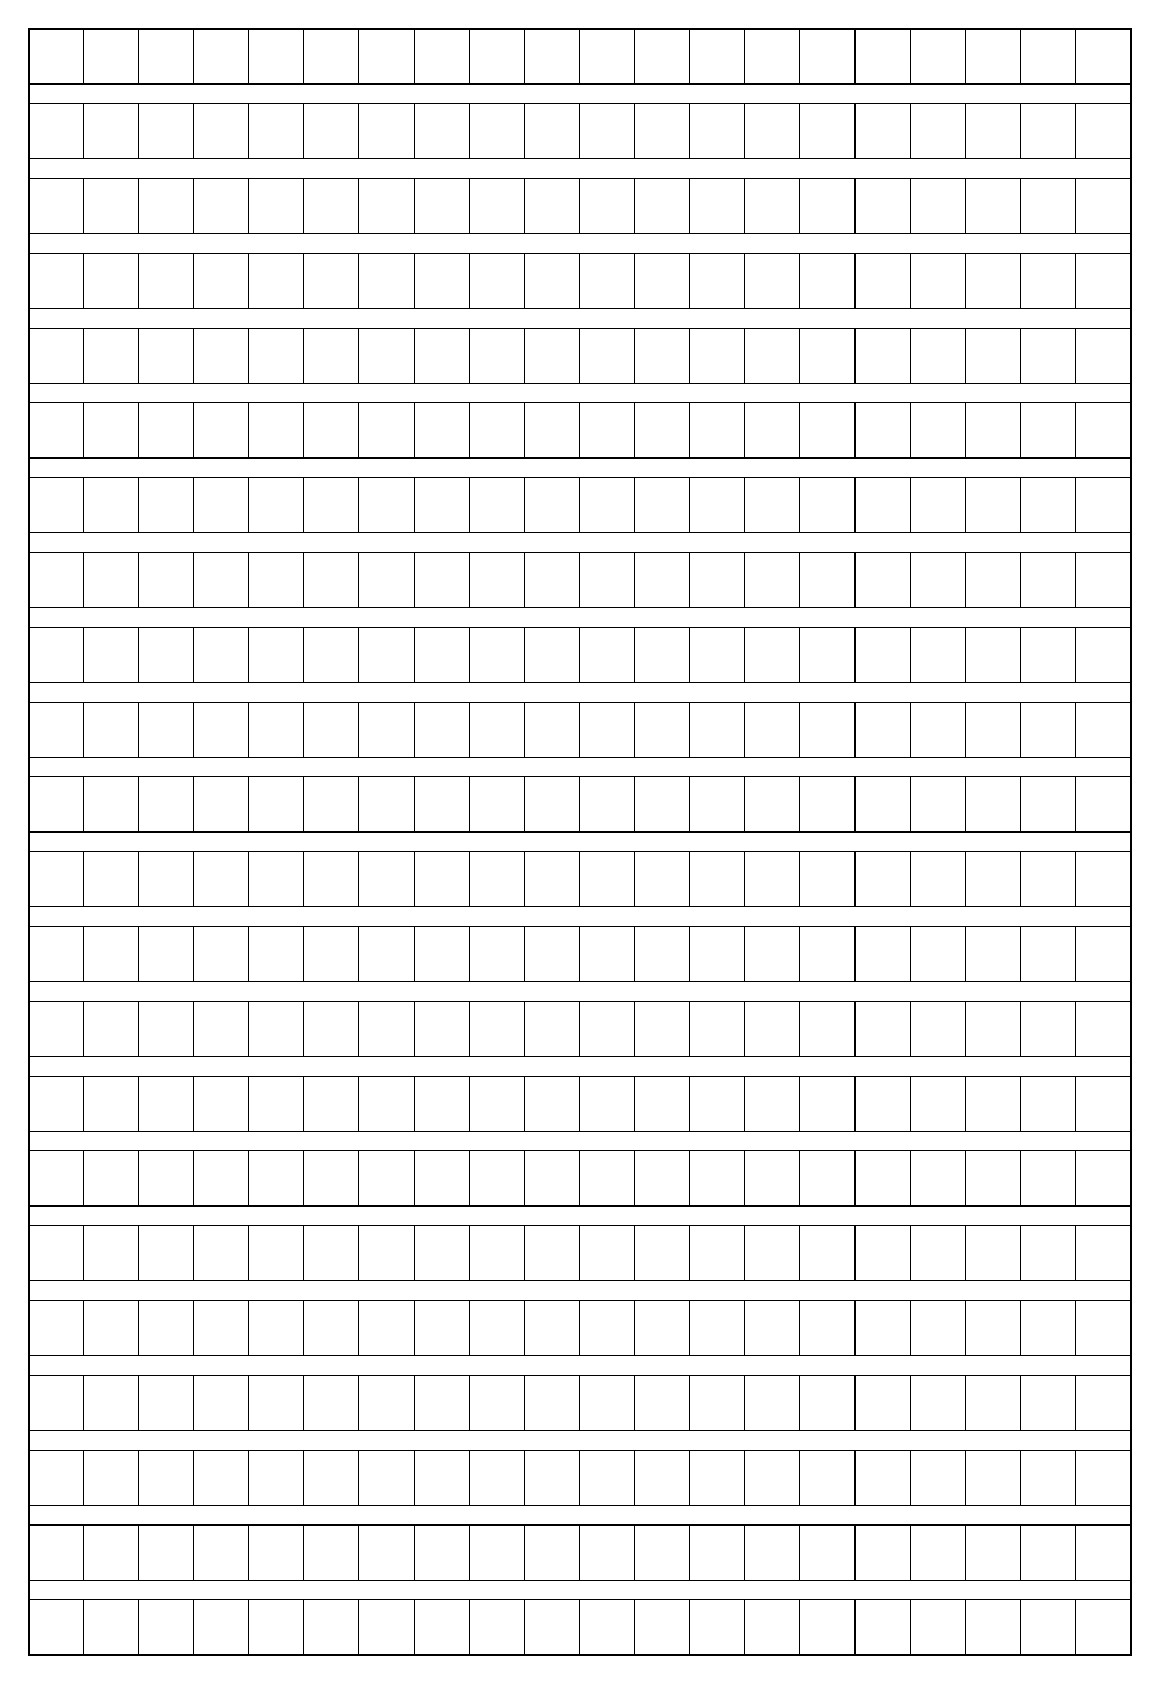
\begin{tikzpicture}[scale=1,x=0.7cm,y=0.95cm]
                \foreach \x [count=\xi] in {1,2,...,20}
                \foreach \y [count=\yi] in {1,2,...,22}
                \node[anchor=east,draw,minimum size=0.7cm]at(\x,\y){};%$\y$
                \draw[thick](0,0.63)rectangle(20,22.37);
                \end{tikzpicture}
            \end{center}
    \end{tcolorbox}
    \end{minipage}

\end{document}